
\begin{exercice}[Coloriage]
Reproduis et colorie le minimum de cases pour que la figure obtenue soit symétrique par rapport aux deux axes rouges :
\begin{center} 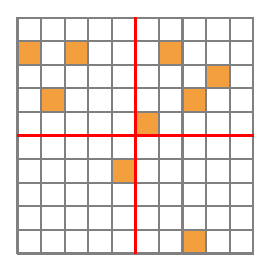
\includegraphics[width=4.2cm]{coloriage_carre} \end{center}
\end{exercice}


\begin{exercice}[Une nouvelle construction]
\begin{enumerate}
 \item Trace à main levée une droite $d$ puis place deux points $M$ et $N$ sur $d$ et un point $B$ n'appartenant pas à $d$ ;
 \item Place, toujours à main levée, le point $B'$ symétrique de $B$ par rapport à $d$ ;
 \item Que peux‑tu dire de $MB$ et $MB'$ ? Justifie ta réponse et code la figure ;
 \item Que peux‑tu dire de $NB$ et $NB'$ ? Justifie ta réponse et code la figure ;
 \item Déduis‑en une méthode de construction du point $B'$ avec tes instruments de géométrie ;
 \item Trace la figure avec tes instruments de géométrie.
 \end{enumerate}
\end{exercice}


\begin{exercice}[L'axe invisible]
\begin{center} 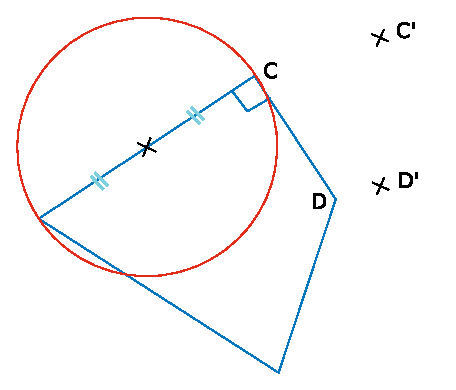
\includegraphics[width=7.2cm]{axe_invisible} \end{center}
Reproduis la figure ci‑dessus. Les points $C'$ et $D'$ sont les symétriques respectifs des points $C$ et $D$ par rapport à un axe invisible. \\[0.5em]
Construis les symétriques du cercle orange et du quadrilatère bleu par rapport à cet axe invisible.
\end{exercice}


\begin{exercice}[Mandala]
\begin{enumerate}
 \item Dessine un cercle de rayon 6 cm et deux de ses diamètres perpendiculaires. Tu obtiens quatre points sur le cercle. Trace tous les axes de symétrie de cette nouvelle figure. Tu obtiens de nouveaux points sur le cercle.
 \item Quel polygone obtiens‑tu en reliant tous ces points ? Combien a‑t‑il d'axes de symétrie ? Trace‑les tous.
 \item Poursuis en traçant un cercle de rayon 3 cm de même centre que celui de 6 cm. Reproduis le motif comme indiqué sur la figure 1 puis termine la construction et le coloriage en faisant des symétries successives par rapport aux axes (voir figure 2).
 \end{enumerate}
 \begin{minipage}[c]{0.48\linewidth}
 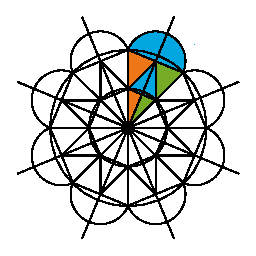
\includegraphics[width=4cm]{mandala1}
 \end{minipage} \hfill%
 \begin{minipage}[c]{0.48\linewidth}
 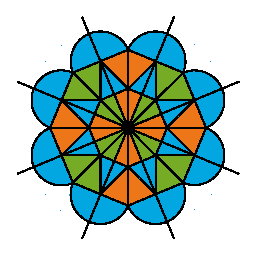
\includegraphics[width=4cm]{mandala2} 
  \end{minipage} \\
\begin{minipage}[c]{0.48\linewidth}
\begin{center} figure 1 \end{center}
 \end{minipage} \hfill%
 \begin{minipage}[c]{0.48\linewidth}
\begin{center} figure 2 \end{center}
  \end{minipage} \\
\end{exercice}


\begin{exercice}[Sans figure]
Melinda a réalisé une superbe figure et son symétrique. Malheureusement, elle a perdu sa feuille, mais sur son cahier, elle avait pris la précaution de faire le tableau suivant :
\begin{center}
\begin{tabularx}{0.9\linewidth}{|c|X|X|X|X|X|X|}
\hline
Points & E & T & R & S & A & C \\ \hline
Symétriques & V & J & I & S & Z & D\\ \hline
 \end{tabularx}
 \end{center}
Frédérique lui fait remarquer qu'avec un tel tableau, on peut obtenir des indications sans avoir besoin de la figure.
\begin{enumerate}
 \item Quel est le centre de la symétrie ?
 \item On sait que $ET = 3,4$ cm et $ZD = 5,1$ cm. Donne les longueurs $AC$ et $VJ$. Justifie.
 \item $RSA$ est un triangle équilatéral de 3 cm de côté. Quel autre triangle équilatéral est-on certain d'avoir sur la figure ? Justifie.
 \item On sait que $VJ = JI$. Quelle est la nature du triangle $ETR$ ? Pourquoi ?
 \end{enumerate}
\end{exercice}


\begin{exercice}[Symétrie et repère]
\begin{enumerate}
 \item Dessine un repère d'origine $O$ ayant pour unité le centimètre.
 \item Place les points : $I (1 ; 0)$ ; $A (2 ; 3)$ ; $B (6 ; - 1)$ ; $C (7 ; 3)$ ; $D (- 1 ; 1)$ ; $E (3 ; 0)$.
 \item Construis les points $F$, $G$, $H$ et $K$, symétriques respectifs de $A$, $B$, $C$ et $D$ par rapport à $O$.
 \item Donne les coordonnées de $F$, $G$, $H$ et $K$. Que remarques-tu ? \label{SymAxCent_approf}
 \item Donne les coordonnées des symétriques par rapport à $O$ des points $T (4 ; - 5)$ et $U (5 ; 0)$ sans les placer dans le repère.
 \item Place les points $M$, $N$, $P$ et $R$, symétriques respectifs des points $A$, $B$, $C$ et $D$ par rapport à $E$.
 \item Donne les coordonnées de $M$, $N$, $P$ et $R$. La propriété de la question \ref{SymAxCent_approf}. se vérifie-t-elle ici ? À quelle condition fonctionne-t-elle ?
 \end{enumerate}
\end{exercice}


\begin{exercice}
Reproduis la figure ci-dessous :
\begin{center} 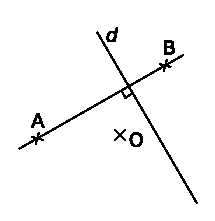
\includegraphics[width=3cm]{croixAOBd} \end{center}
\begin{enumerate}
 \item Construis les points $E$ et $F$, symétriques respectifs de $A$ et $B$ par rapport à $O$.
 \item Que peut-on dire des droites $(AB)$ et $(EF)$ ? Justifie ta réponse.
 \item Démontre que les droites $d$ et $(EF)$ sont perpendiculaires.
 \end{enumerate}
\end{exercice}


\begin{exercice}[Médiatrice et symétrie]
\begin{enumerate}
 \item Trace trois droites $d_1$, $d_2$ et $d_3$, concourantes en un point $O$ puis place :
 \begin{itemize}
  \item Sur $d_1$, $A$ et $A'$ tels que $OA = OA' = 3$ cm ;
  \item Sur $d_2$, $B$ et $B'$ tels que $OB = OB' = 4$ cm ;
  \item Sur $d_3$, $C$ et $C'$ tels que $OC = OC' = 5$ cm.
  \end{itemize}
 \item Démontre que $(B'C')$ et $(BC)$ sont parallèles.
 \item Construis la médiatrice d du segment $[BC]$.
 \item Démontre que $d$ est perpendiculaire à $(B'C')$.
 \end{enumerate}
\end{exercice}


\begin{exercice}[Pentagone et hexagone]
\underline{PARTIE A}
\begin{enumerate}
 \item Sur un cercle de centre $O$ et de rayon 4 cm, place un point $A$ puis quatre autres points distincts : $B$, $C$, $D$ et $E$ dans cet ordre tels que les angles $\widehat{AOB}$, $\widehat{BOC}$, $\widehat{COD}$, $\widehat{DOE}$ et $\widehat{EOA}$ mesurent tous $72^\circ$. 
 \item Trace le pentagone $ABCDE$. Que penses-tu des longueurs des côtés de ce pentagone ? Ce pentagone est appelé un pentagone régulier. A-t-il un centre de symétrie ?
\underline{PARTIE B}
 \item Sur un autre cercle de centre $O$ et de rayon 4 cm, place six points distincts $A$, $B$, $C$, $D$, $E$ et $F$ dans cet ordre tels que les angles $\widehat{AOB}$, $\widehat{BOC}$, $\widehat{COD}$, $\widehat{DOE}$, $\widehat{EOF}$ et $\widehat{FOA}$ mesurent tous $60^\circ$.
 \item Trace l'hexagone $ABCDEF$. Que penses-tu des longueurs des côtés de cet hexagone ? Cet hexagone est appelé un hexagone régulier. A-t-il un centre de symétrie ?
 \item Trace les triangles $ACE$ et $BDF$. Colorie avec plusieurs couleurs la figure en respectant la symétrie.
 \end{enumerate}
\end{exercice}


